\documentclass[border=16pt,tikz]{standalone}
\usepackage{tikz}
\usetikzlibrary{positioning,arrows.meta,fit,backgrounds,calc}

\definecolor{cext}{RGB}{232,232,232}
\definecolor{cprx}{RGB}{173,216,230}
\definecolor{capp}{RGB}{144,238,144}
\definecolor{cdb} {RGB}{255,228,181}
\definecolor{cphi}{RGB}{255,175,175}
\definecolor{csec}{RGB}{255,192,203}
\definecolor{cobs}{RGB}{216,191,216}

\tikzset{
  nd/.style={draw, rounded corners=5pt,
             minimum width=2.8cm, minimum height=0.9cm,
             font=\small\sffamily, align=center, inner sep=4pt},
  ext/.style={nd, fill=cext,  draw=gray!70},
  prx/.style={nd, fill=cprx,  draw=blue!60},
  app/.style={nd, fill=capp,  draw=green!60!black},
  dbs/.style={nd, fill=cdb,   draw=orange!70},
  phi/.style={nd, fill=cphi,  draw=red!70, line width=1.2pt},
  sec/.style={nd, fill=csec,  draw=red!50},
  obs/.style={nd, fill=cobs,  draw=purple!60},
  arr/.style={-{Stealth[length=6pt,width=5pt]}, semithick, gray!60},
  darr/.style={arr, dashed, gray!50},
  grp/.style={draw, rounded corners=8pt, inner sep=8pt},
}

\begin{document}
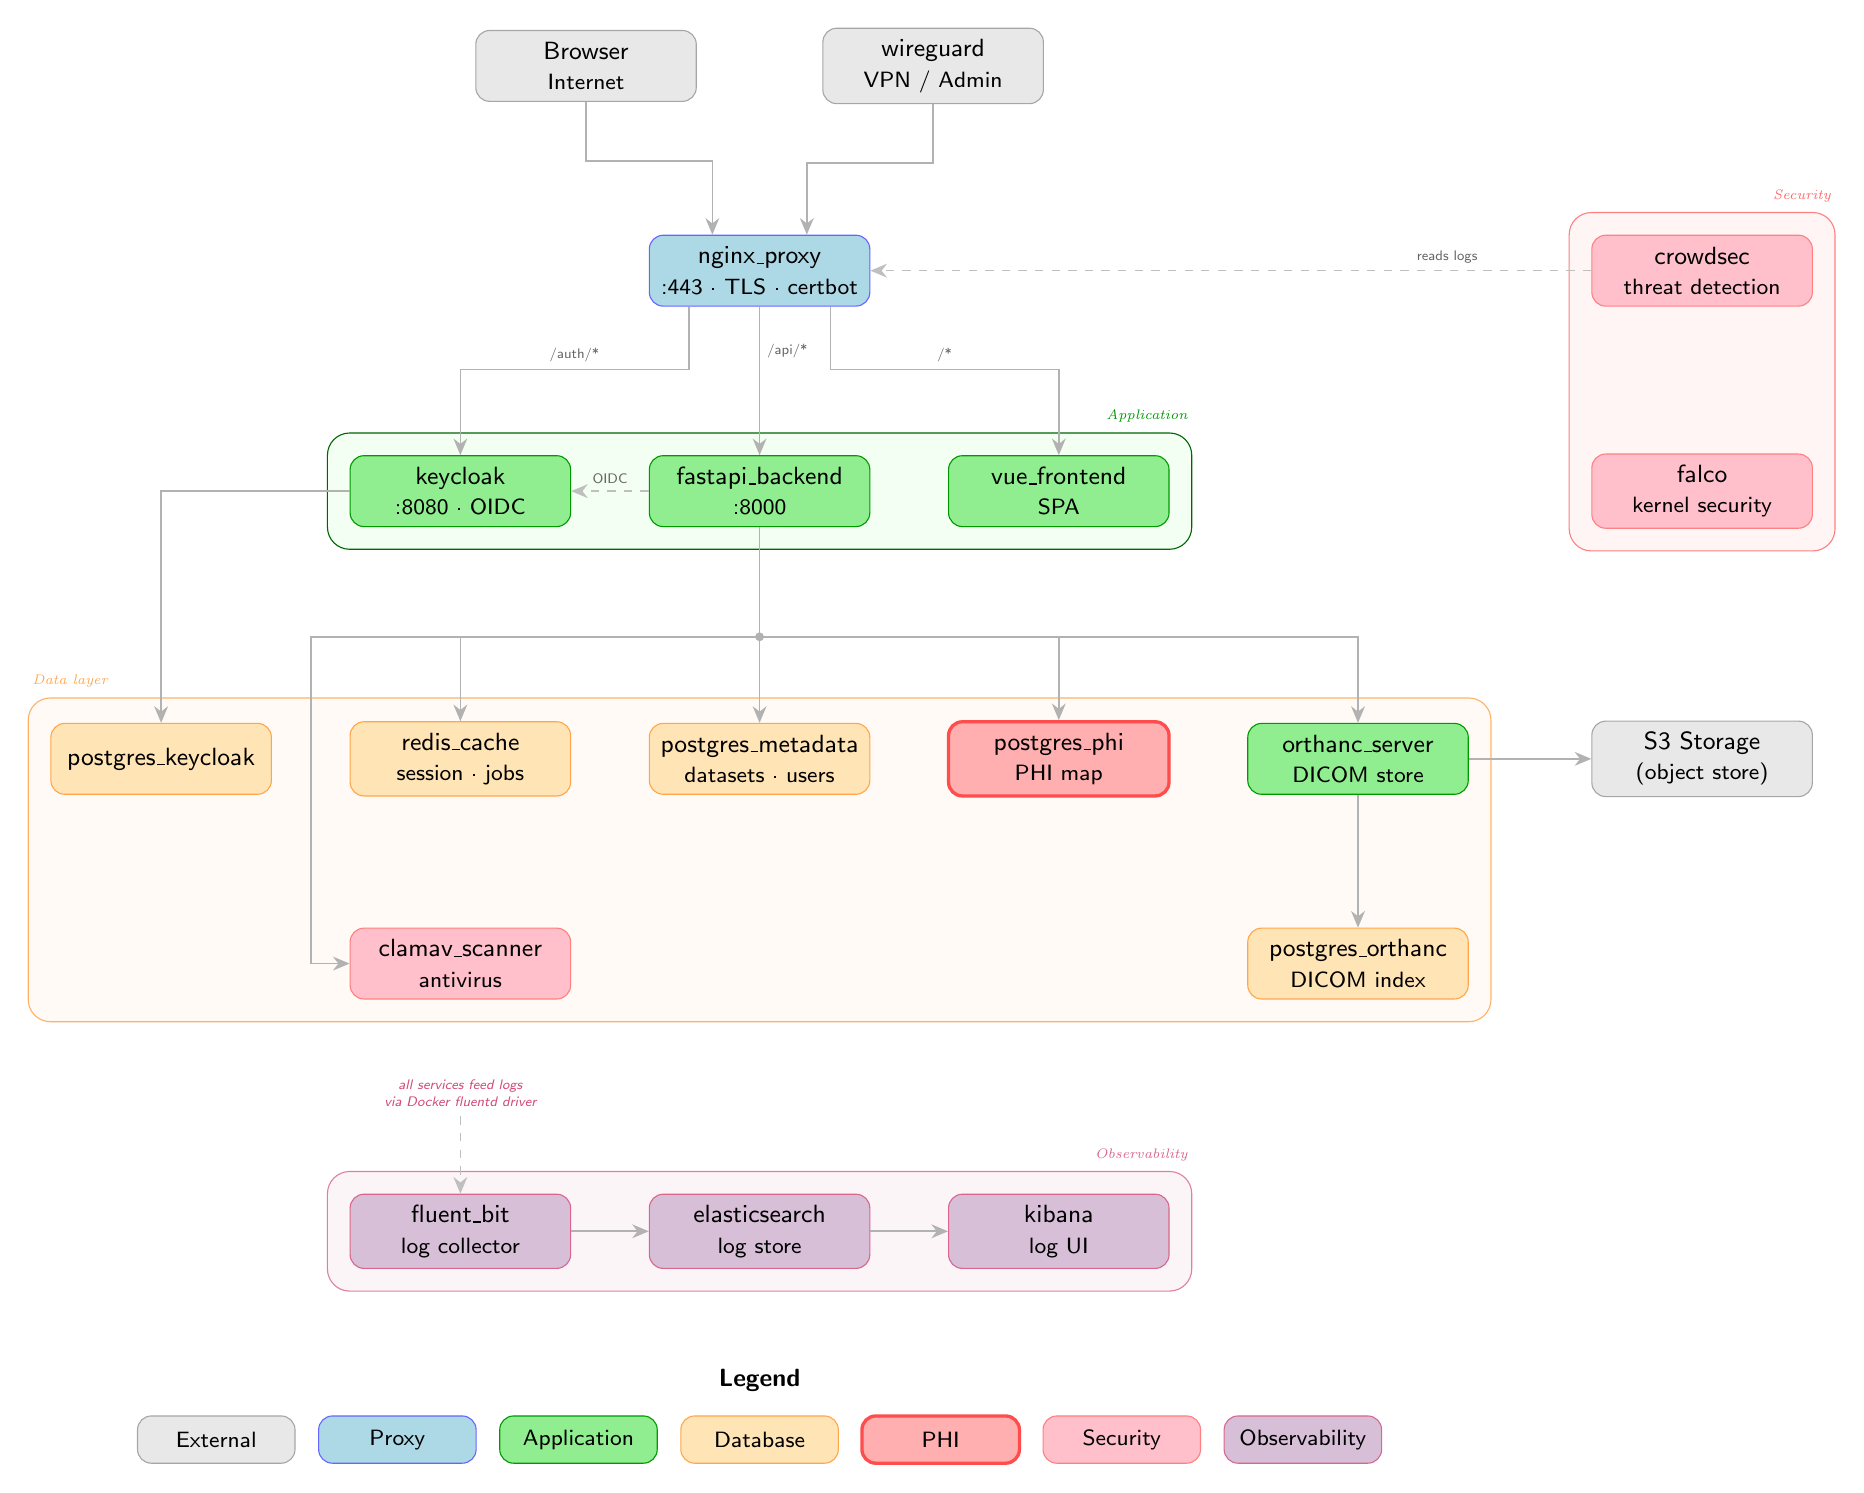
\begin{tikzpicture}
\def\cw{3.8}        % column pitch
\def\yedge{-2.6}    % nginx / crowdsec row
\def\yapp{-5.4}     % application row
\def\ydata{-8.8}    % data row 1
\def\ydatab{-11.4}  % data row 2
\def\yobs{-14.8}    % observability row
\def\ybus{-7.25}    % fastapi fan-out line, between application and data groups

%% ---- External ------------------------------------------------
\node[ext] (browser)   at (1.42*\cw, 0) {Browser\\{\footnotesize Internet}};
\node[ext] (wireguard) at (2.58*\cw, 0) {wireguard\\{\footnotesize VPN / Admin}};

%% ---- Edge ----------------------------------------------------
\node[prx] (nginx) at (2*\cw, \yedge)
  {nginx\_proxy\\{\footnotesize :443 · TLS · certbot}};

%% ---- Application ---------------------------------------------
\node[app] (keycloak) at (1*\cw, \yapp) {keycloak\\{\footnotesize :8080 · OIDC}};
\node[app] (fastapi)  at (2*\cw, \yapp) {fastapi\_backend\\{\footnotesize :8000}};
\node[app] (vue)      at (3*\cw, \yapp) {vue\_frontend\\{\footnotesize SPA}};

%% ---- Data layer ----------------------------------------------
\node[dbs] (pgkc)    at (0*\cw, \ydata) {postgres\_keycloak};
\node[dbs] (redis)   at (1*\cw, \ydata) {redis\_cache\\{\footnotesize session · jobs}};
\node[dbs] (pgmeta)  at (2*\cw, \ydata) {postgres\_metadata\\{\footnotesize datasets · users}};
\node[phi] (pgphi)   at (3*\cw, \ydata) {postgres\_phi\\{\footnotesize PHI map}};
\node[app] (orthanc) at (4*\cw, \ydata) {orthanc\_server\\{\footnotesize DICOM store}};

\node[sec] (clamav)    at (1*\cw, \ydatab) {clamav\_scanner\\{\footnotesize antivirus}};
\node[dbs] (pgorthanc) at (4*\cw, \ydatab) {postgres\_orthanc\\{\footnotesize DICOM index}};
\node[ext] (s3)        at (5.15*\cw, \ydata) {S3 Storage\\{\footnotesize (object store)}};

%% ---- Security ------------------------------------------------
\node[sec] (crowdsec) at (5.15*\cw, \yedge) {crowdsec\\{\footnotesize threat detection}};
\node[sec] (falco)    at (5.15*\cw, \yapp)  {falco\\{\footnotesize kernel security}};

%% ---- Observability -------------------------------------------
\node[obs] (fluentbit) at (1*\cw, \yobs) {fluent\_bit\\{\footnotesize log collector}};
\node[obs] (elastic)   at (2*\cw, \yobs) {elasticsearch\\{\footnotesize log store}};
\node[obs] (kibana)    at (3*\cw, \yobs) {kibana\\{\footnotesize log UI}};

%% ==== ARROWS =================================================
\tikzset{elbl/.style={font=\tiny\sffamily, text=gray!80!black, inner sep=2.5pt}}

%% External -> nginx (two separate entry points on the top edge)
\draw[arr] (browser.south)   -- ++(0,-0.75) -| ([xshift=-6mm]nginx.north);
\draw[arr] (wireguard.south) -- ++(0,-0.75) -| ([xshift=6mm]nginx.north);

%% nginx -> apps (three separate exits on the bottom edge)
\draw[arr] (nginx.south) -- node[elbl, right, pos=0.3]{/api/*} (fastapi.north);
\draw[arr] ([xshift=-9mm]nginx.south) -- ++(0,-0.8)
  -| node[elbl, above, pos=0.25]{/auth/*} (keycloak.north);
\draw[arr] ([xshift=9mm]nginx.south) -- ++(0,-0.8)
  -| node[elbl, above, pos=0.25]{/*} (vue.north);

%% FastAPI -> Keycloak (OIDC token verify, dashed)
\draw[darr] (fastapi.west) -- node[elbl, above]{OIDC} (keycloak.east);

%% Keycloak -> postgres_keycloak (leaves on the left, clear of the fan-out)
\draw[arr] (keycloak.west) -| (pgkc.north);

%% FastAPI fan-out: one trunk, one horizontal line, one drop per target
\coordinate (bus) at (fastapi.south |- 0,\ybus);
\draw[arr] (fastapi.south) -- (pgmeta.north);
\draw[arr] (bus) -| (redis.north);
\draw[arr] (bus) -| (pgphi.north);
\draw[arr] (bus) -| (orthanc.north);
%% ClamAV: down the free lane between the first two columns
\draw[arr] (bus) -| ($(pgkc.east)!0.5!(redis.west) + (0,-0.4)$) |- (clamav.west);
\fill[gray!60] (bus) circle (1.6pt);

%% Orthanc -> storage
\draw[arr] (orthanc.south) -- (pgorthanc.north);
\draw[arr] (orthanc.east)  -- (s3.west);

%% CrowdSec reads nginx logs
\draw[darr] (crowdsec.west) -- node[elbl, above, pos=0.2]{reads logs} (nginx.east);

%% Observability chain
\draw[arr] (fluentbit) -- (elastic);
\draw[arr] (elastic)   -- (kibana);

%% Logging note (all services -> fluent_bit via Docker logging driver)
\node[font=\tiny\sffamily\itshape, text=purple!70, align=center] (lognote)
  at (1*\cw, \yobs+1.75) {all services feed logs\\via Docker fluentd driver};
\draw[darr] (lognote.south) -- (fluentbit.north);

%% ==== BACKGROUND GROUPS =====================================
\begin{pgfonlayer}{background}
  \node[grp, draw=green!40!black, fill=green!5,
        fit=(fastapi)(keycloak)(vue)] (gapp) {};
  \node[grp, draw=orange!60, fill=orange!4,
        fit=(redis)(pgmeta)(pgphi)(pgkc)(orthanc)(clamav)(pgorthanc)] (gdata) {};
  \node[grp, draw=red!50, fill=red!4,
        fit=(crowdsec)(falco)] (gsec) {};
  \node[grp, draw=purple!50, fill=purple!4,
        fit=(fluentbit)(elastic)(kibana)] (gobs) {};
\end{pgfonlayer}
\tikzset{glbl/.style={font=\tiny\itshape, inner sep=1.5pt}}
\node[glbl, green!60!black, anchor=south east] at ([yshift=2pt]gapp.north east)  {Application};
\node[glbl, orange!70,      anchor=south west] at ([yshift=2pt]gdata.north west) {Data layer};
\node[glbl, red!60,         anchor=south east] at ([yshift=2pt]gsec.north east)  {Security};
\node[glbl, purple!60,      anchor=south east] at ([yshift=2pt]gobs.north east)  {Observability};

%% ==== LEGEND ================================================
\begin{scope}[shift={($(gdata.south)+(-6.9,-5.3)$)}]
  \node[font=\small\sffamily\bfseries] at (6.9, 0.75) {Legend};
  \foreach \lbl/\sty/\xx in {
    External/ext/0,
    Proxy/prx/2.3,
    Application/app/4.6,
    Database/dbs/6.9,
    PHI/phi/9.2,
    Security/sec/11.5,
    Observability/obs/13.8}
  {
    \node[\sty, minimum width=2.0cm, minimum height=0.6cm,
          font=\footnotesize\sffamily] at (\xx,0) {\lbl};
  }
\end{scope}

\end{tikzpicture}
\end{document}
